%!TEX root = main.tex

Figure\ref{fig.method} illustrates our technical approach.   
%
The top row shows the steps of the training process.  First training images are preprocessed using data augmentation techniques to increase data diversity. 
The augmented data are fed into deep convolutional neural network(ConvNet) for training. The trained deep ConvNet then serves as a feature extractor for a support vector machine (SVM) which uses the deep features from the trained deep ConvNet as input, and is trained to classify the pattern type.
%
During the testing, shown in the bottom row of Figure\ref{fig.method}, testing images are fed into the trained deep ConvNet for deep features extraction. These intermediate deep features are used as input features to the trained SVM. The output of the SVM is final pattern class predictions.


\begin{figure}[!ht]
	\begin{center}
		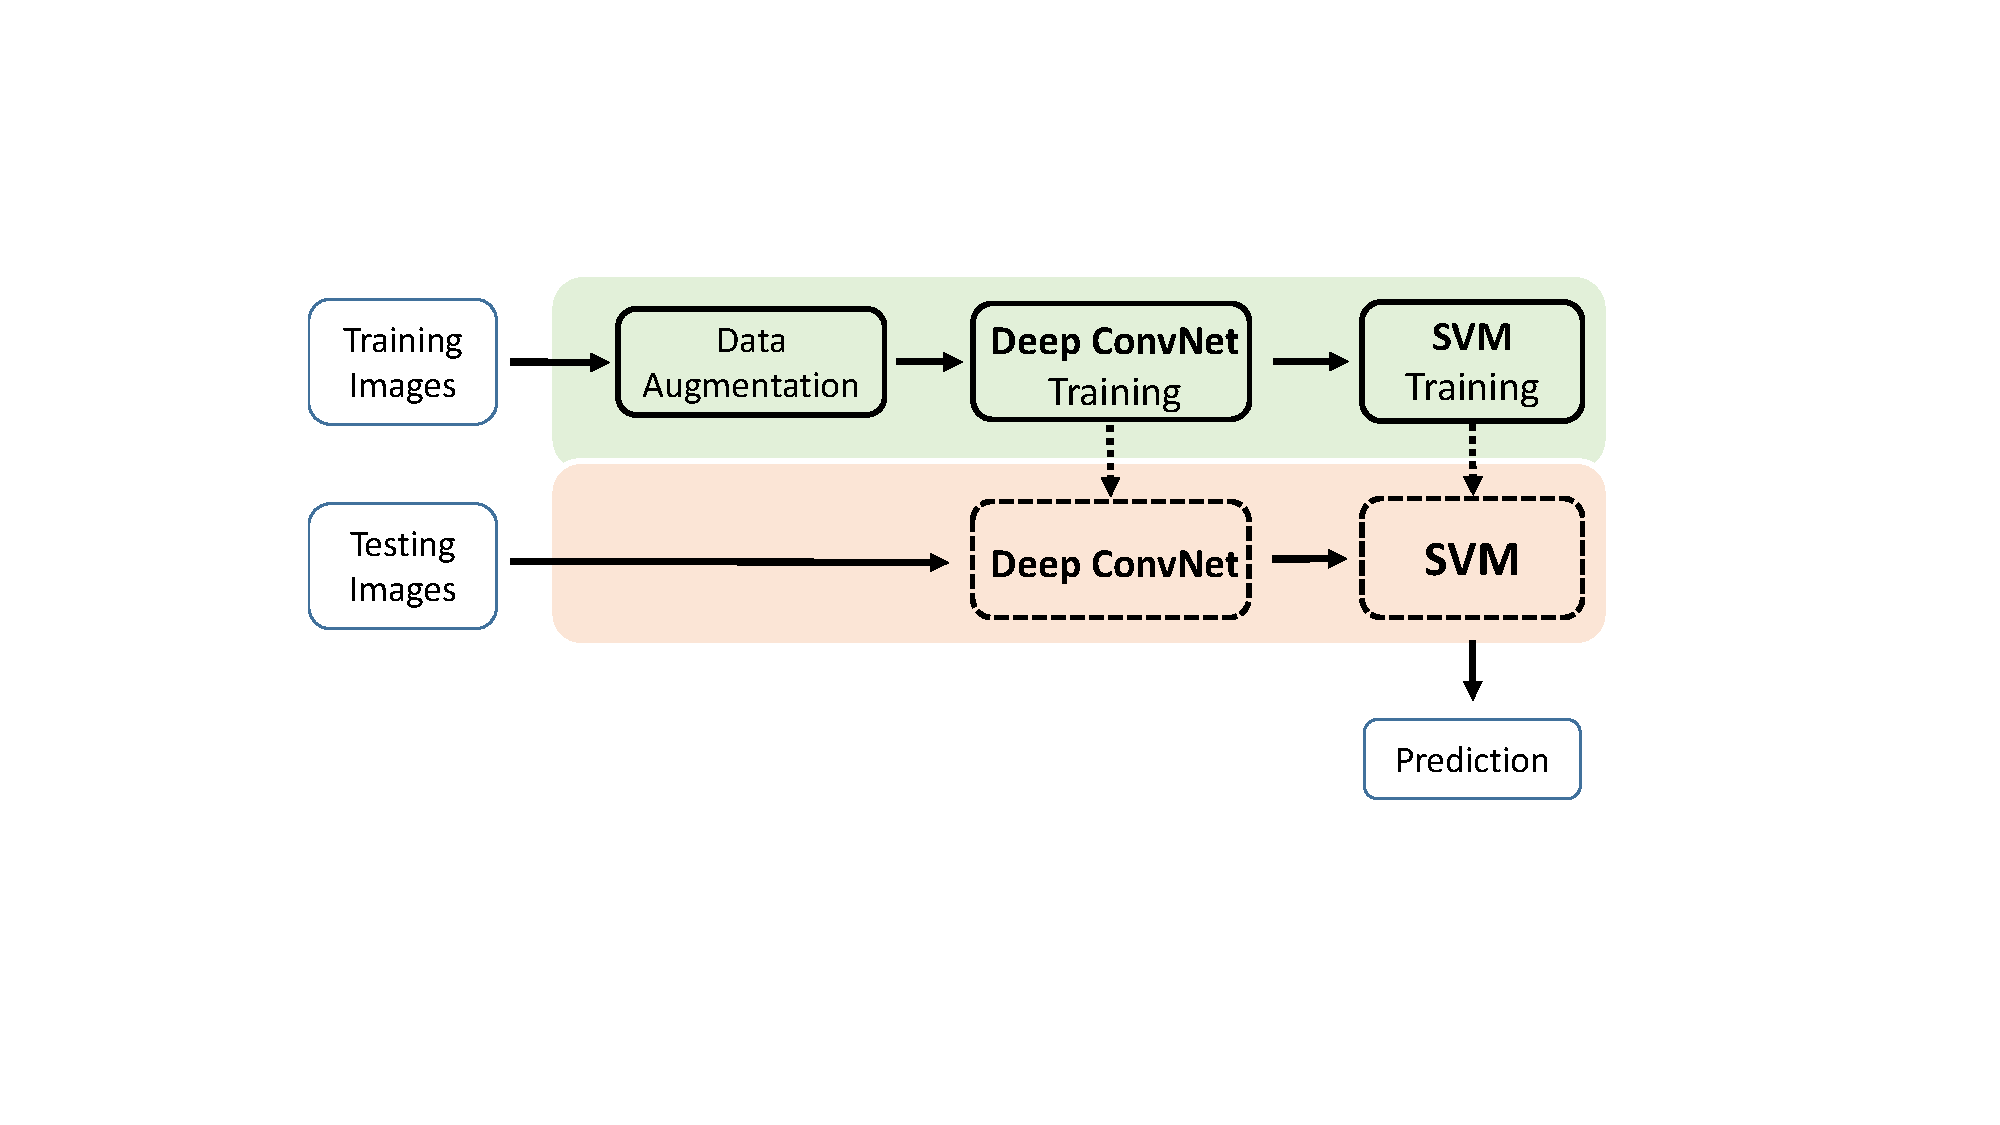
\includegraphics[scale=0.38,clip=true,trim = 50mm 55mm 28mm 50mm]{fig/figs/method_overview.pdf}
	\end{center}
	\caption{Overview of proposed approach.} 
	\label{fig.method}
\end{figure}

%-------------------------
\subsection{Deep ConvNet Architecture}
\label{sec_cnn}
Our proposed network architecture (Figure \ref{fig.cnn_arch})  is based on deep residual network proposed by Kaiming He \textbf{et al.}\cite{he2016deep}. Deep residual  network has been proven to outperform other deep plain networks because it addresses the degradation problem by reformulating the layers as learning residual functions instead of learning unreferenced functions. 
%
Table\ref{tab.cnn_params} summarizes the details of our network. The input size of our deep ConvNet is $512\times512$ and the number of channels is $1$.
The first two layers of our network are convolutional layers which has 96 $7\times7$ filters and the stride is 2. The third layer has 64 $7\times7$ filters and the stride is 2. 
%
\textit{conv4}, \textit{conv5}, \textit{conv6} and \textit{conv7} are composed of residual building blocks. Specifically, there is a max pooling layer before  \textit{conv4}. The parameters inside the brackets specify the residual building block size. 
%
The multiplier after bracket specifies the multiplicity of the that block in that layer.  More details and explanations regarding network architecture can be found in \cite{he2016deep}. 
%
The global pooling layer in \textit{conv8} generates $1\times1,2048$ output and the last layer uses 5 $1\times1$ filters to generate the final prediction. 
%
The number of parameters of proposed deep ConvNet is $24.26$ million. 
%
We use Relu\cite{nair2010rectified} as intermediate activation function.
%

The novelty of our network is that we use $512\times512$ as network input size. This preserves the detail of fingerprint to the extent possible. 
%
However, the larger the size of input images, the larger the computational cost.  We empirically searched for the optimal input image size and we found that the performance drops as the size gets smaller, and it drops significantly for images smaller than $224\times224$ -- as shown in Figure\ref{fig.resize_examples}, down-sampling the images to $224\times224$, results in loss of information content of prints and reduces the clarity of ridge details and deltas and cores. 
%
Therefore we decided against significant down sampling.  
%
We also ruled out cropping or segmenting the fingerprint portion of an image, that is removing background and non-fingerprint portion of images to get smaller images, because of its requiring to employ a segmentation algorithm and reliance on the accuracy of the segmentation algorithm -- recall that one of our objective has been to avoid fingerprint processing and characterization.
%
After careful visual inspection of fingerprint images of different sizes, we decided to use $512\times512$ as input size for the following reasons. 
%
First, sufficient fingerprint detail is preserved at this size. Second, it is a reasonable size for rolled fingerprints. Finally, it is the original image size of one of the datasets we used, which is NIST SD4. 
To remedy the huge computational cost and high memory usage during the training, we added \textit{conv1} and \textit{conv2} with stride 2 to down-sample the input images. As shown in Table.\ref{tab.cnn_params}, after \textit{conv2}, the feature map size is $128\times128, 96$. So, the spatial size is reduced (from $512 \times 512$ to $128 \times 128$) and spatial information is stored in the increased channels (from $1$ to $96$).

%
\begin{figure}[!ht]
	\begin{center}
		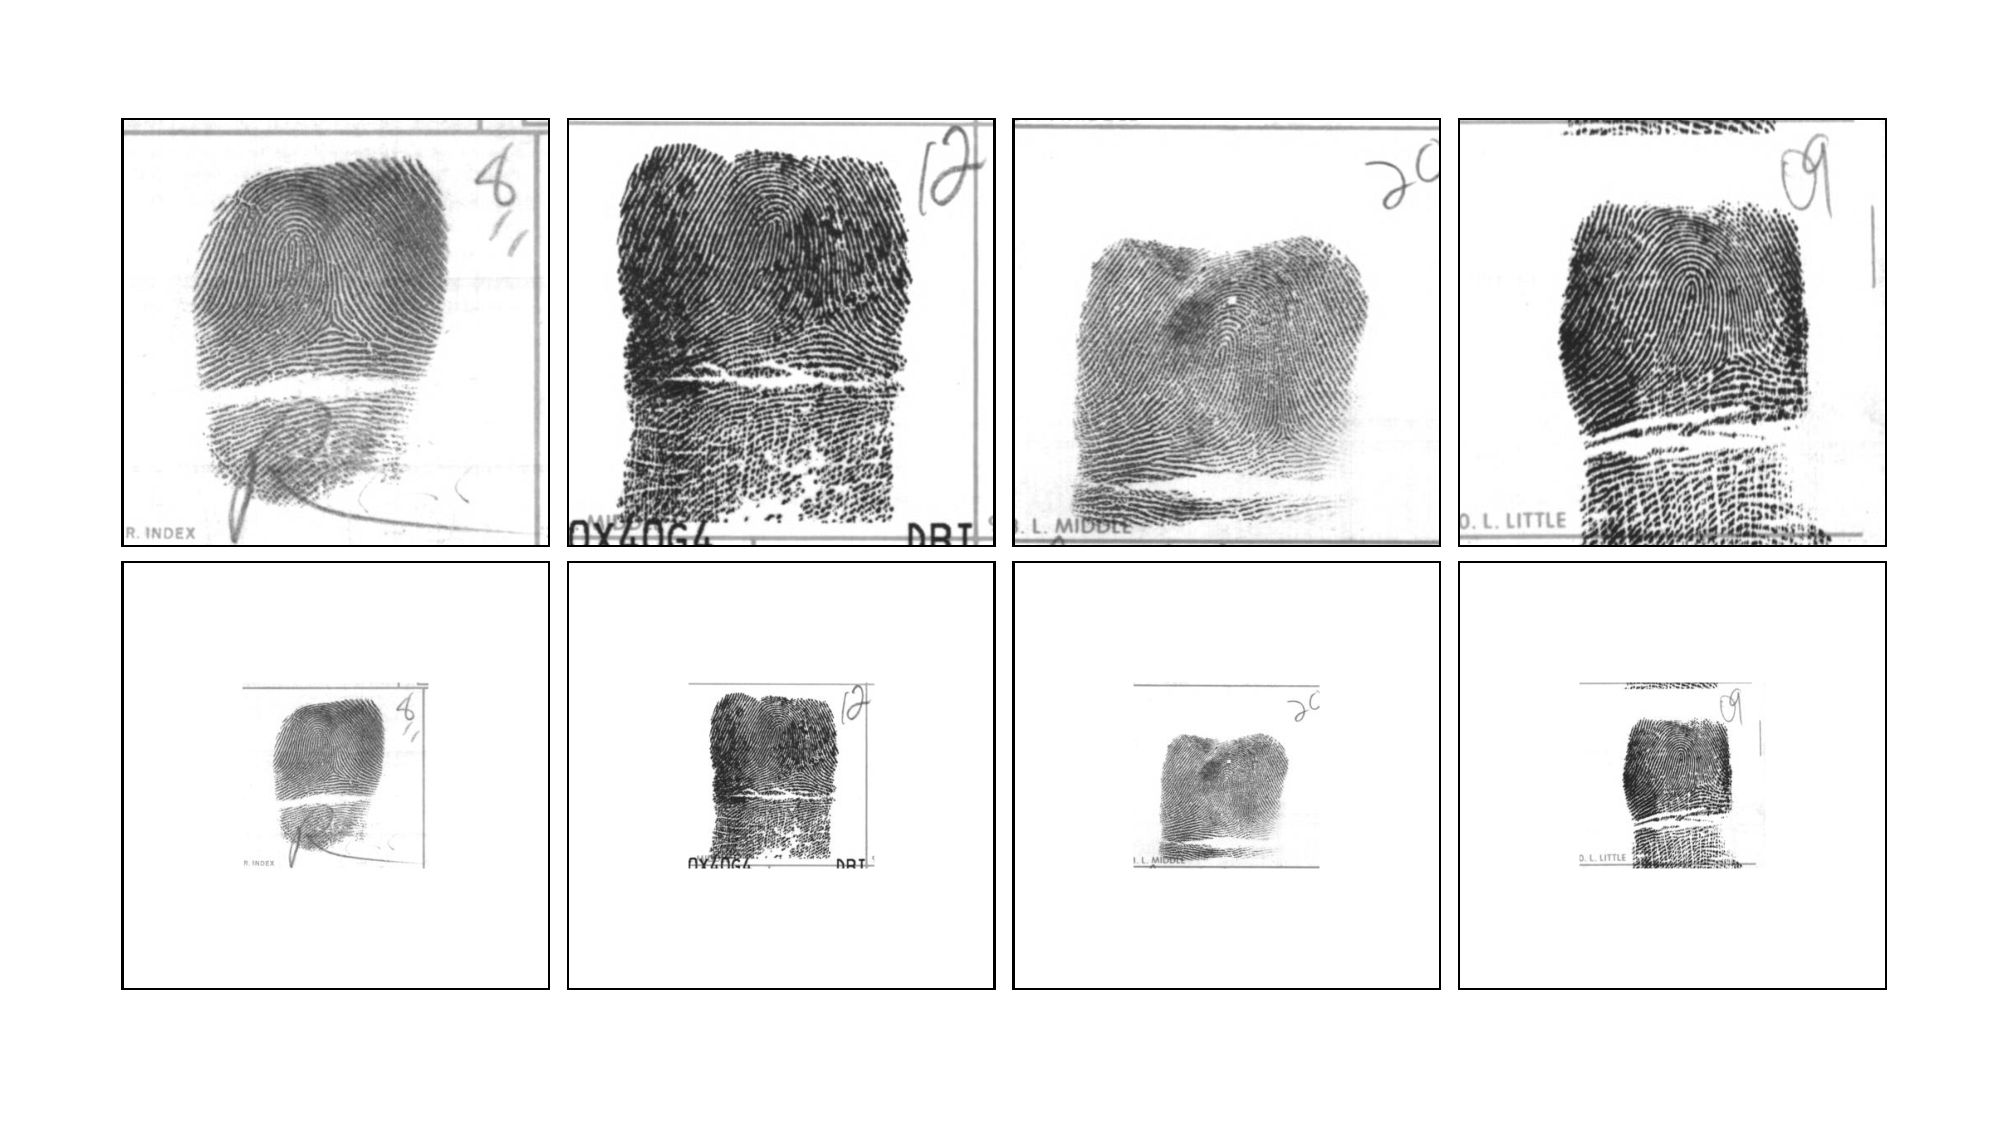
\includegraphics[scale=0.28,clip=true,trim = 20mm 15mm 10mm 10mm]{fig/figs/resize_examples.pdf}
	\end{center}
	\caption{Example images from NIST SD14 with different spatial sizes. The top row images are $512\times512$ and the bottom row are $224\times224$. Ridges of top images are more distinguishable than that of bottom images. } 
	\label{fig.resize_examples}
\end{figure}
%
%
\begin{figure*}[!ht]
	\begin{center}
		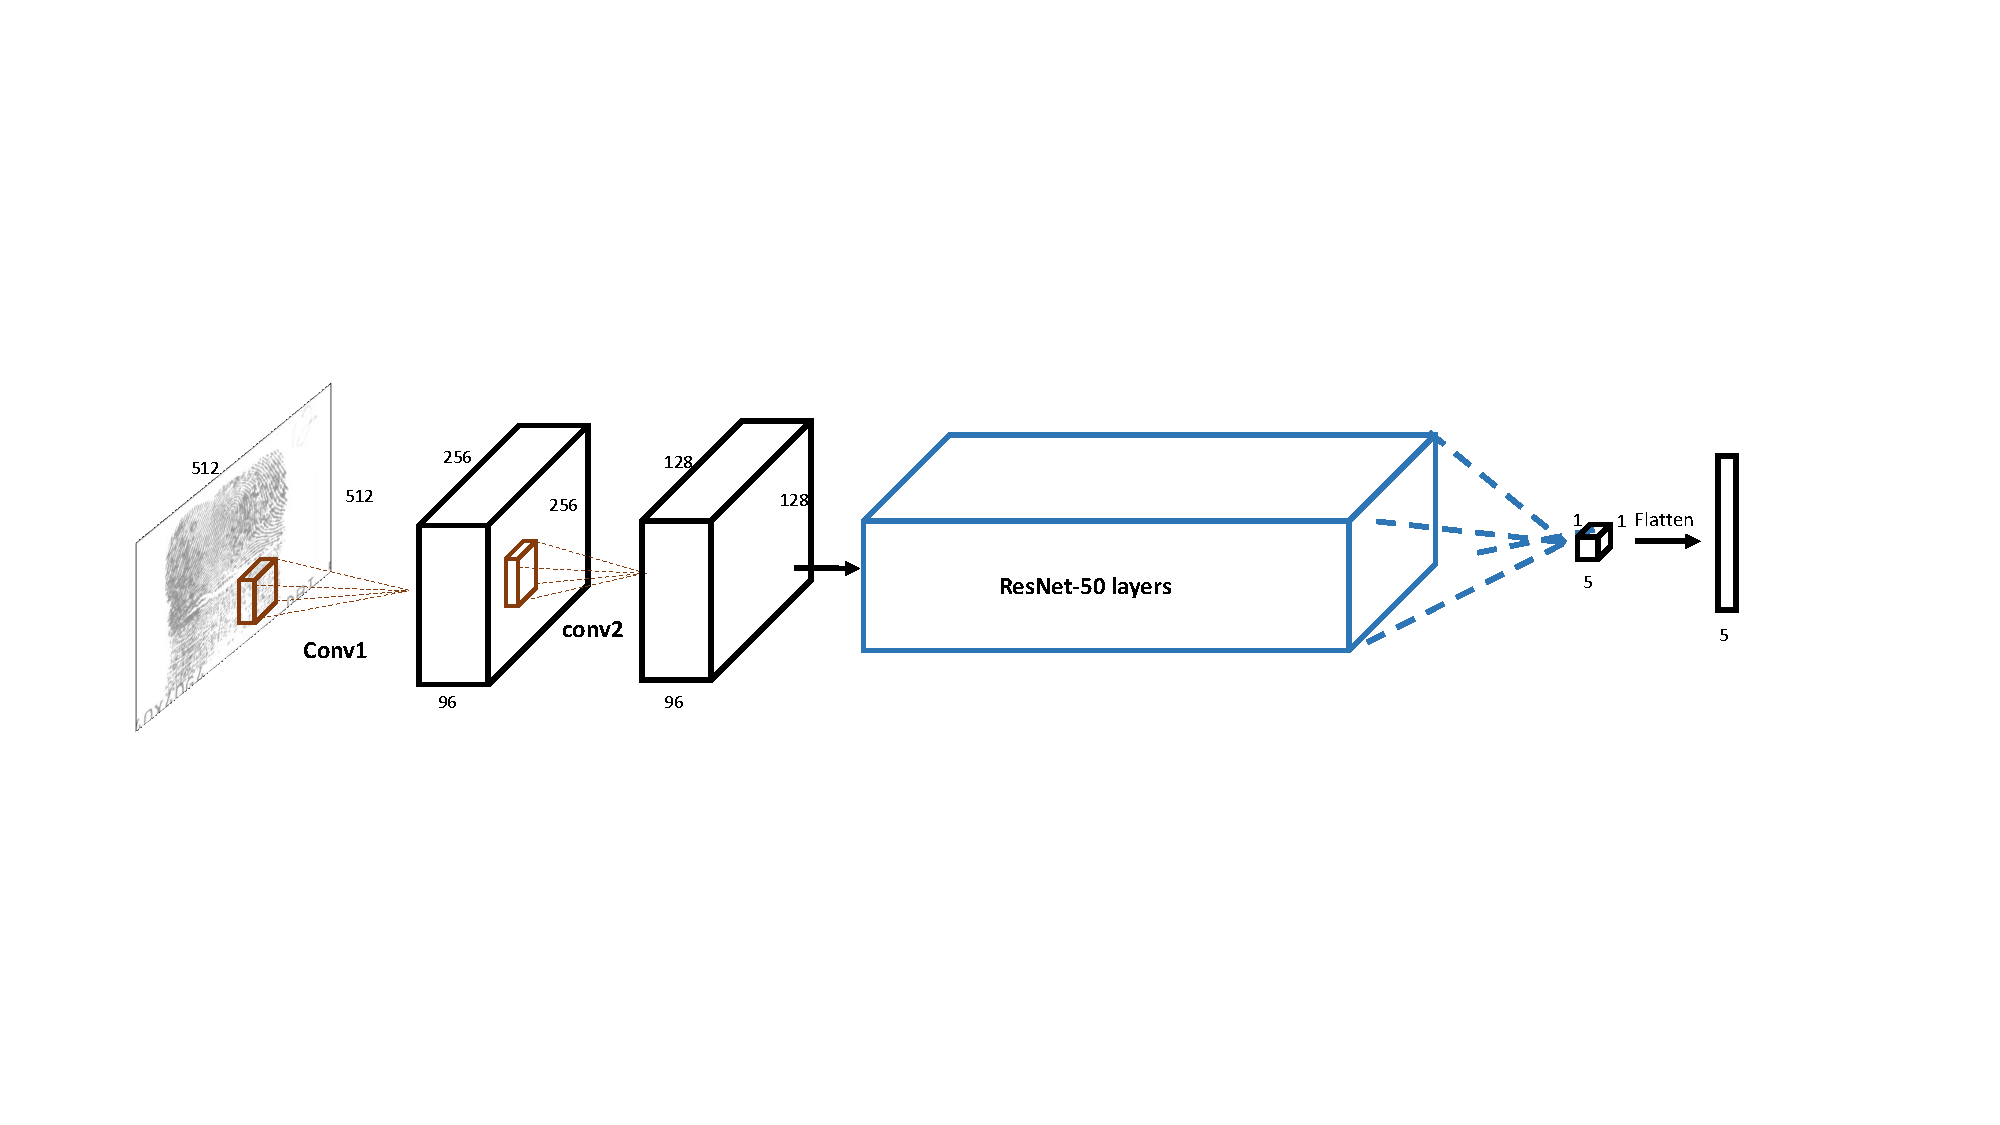
\includegraphics[scale=0.65,clip=true,trim = 20mm 65mm 30mm 65mm]{fig/figs/cnn_arch.pdf}
	\end{center}
	\caption{Architecture of proposed CNN.} 
	\label{fig.cnn_arch}
\end{figure*}


\begin{table}[!ht]
	\centering
	\caption{Detail of proposed deep ConvNet. The format is inspired by \cite{he2016deep}}
	\label{tab.cnn_params}
	\begin{tabular}{l}
		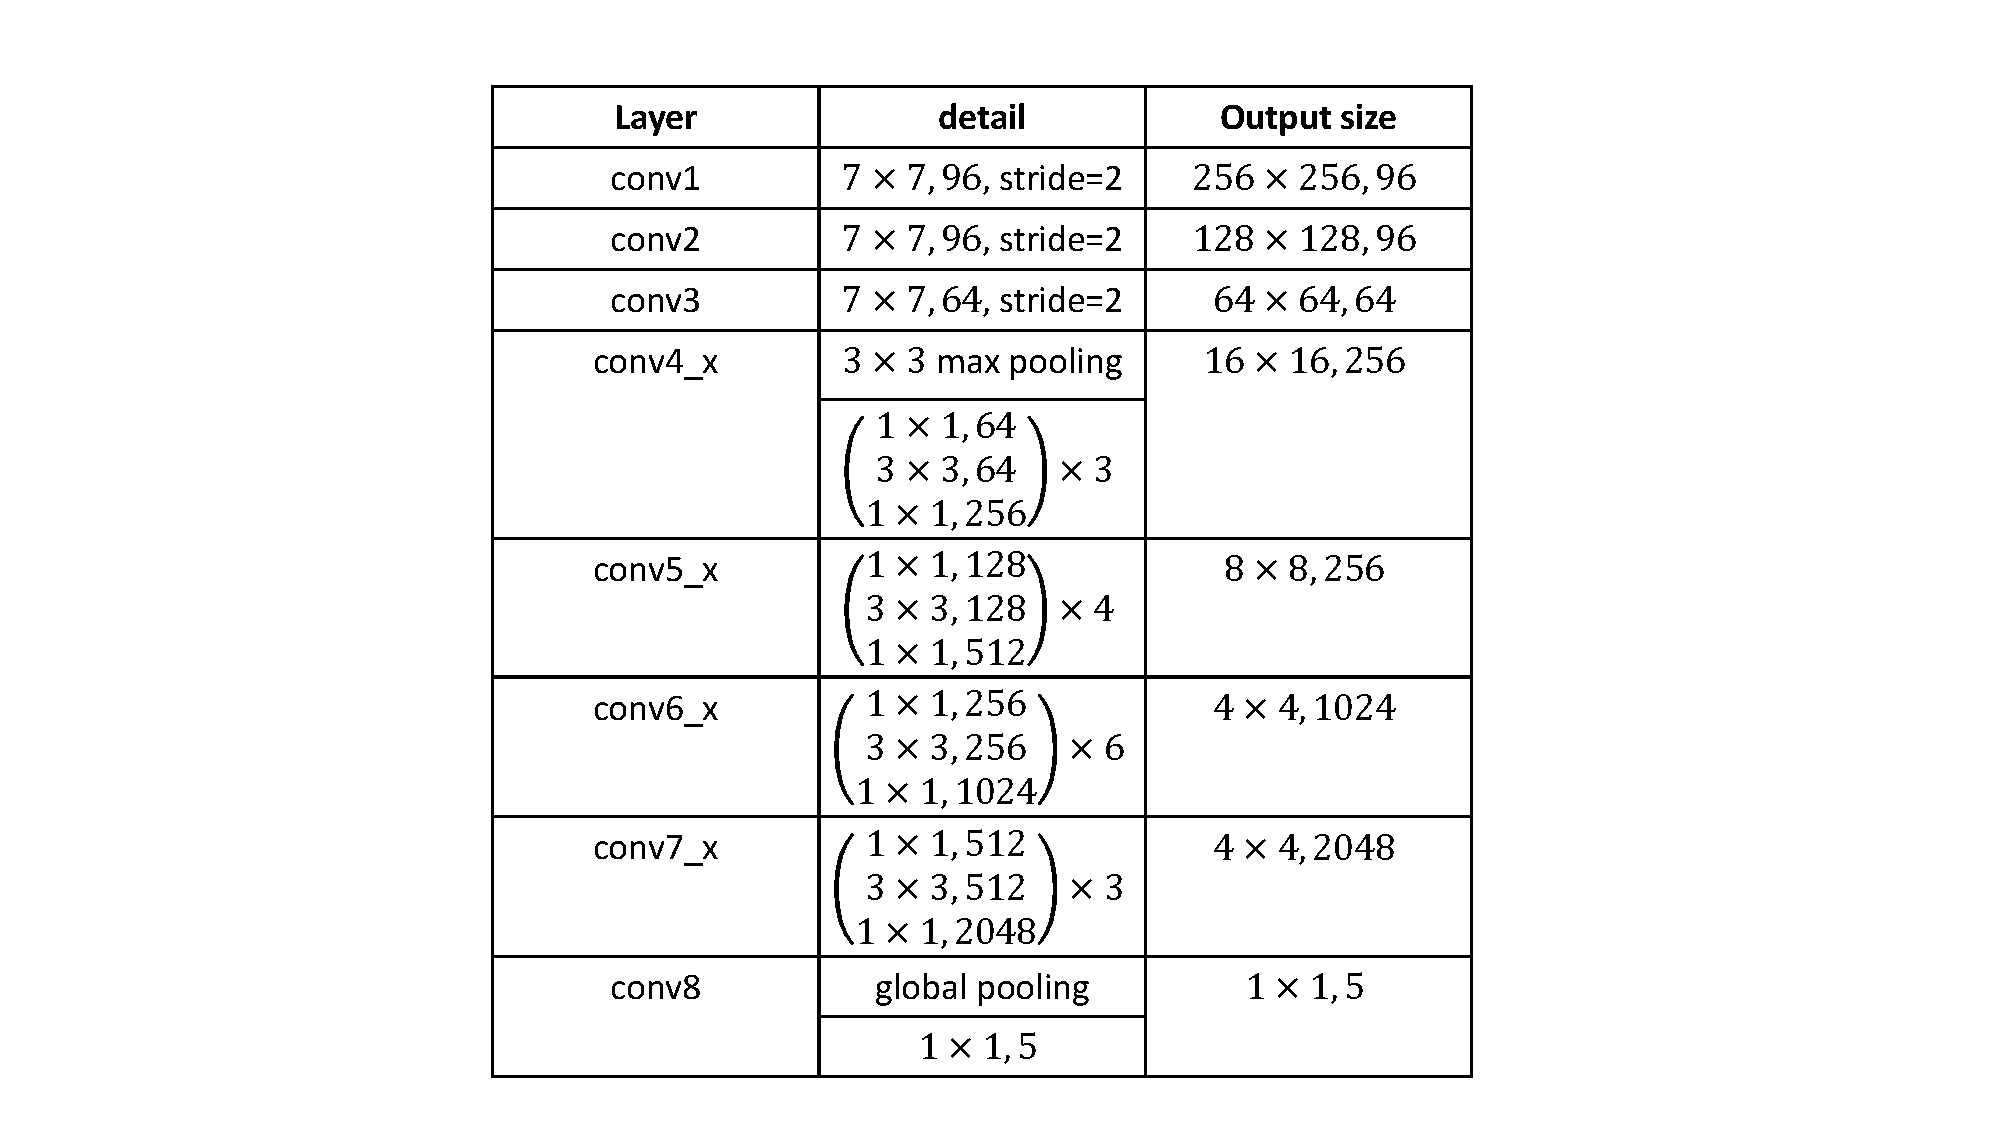
\includegraphics[scale=0.45,clip=true,trim = 78mm 5mm 70mm 5mm]{fig/figs/cnn_table.pdf}
	\end{tabular}
\end{table}

%-------------------------
\subsection{Data Augmentation}
\label{sec-dataAug}
Fingerprint images exhibit a wide range of location, rotation, brightness and contrast. To enhance the generalization ability of our ConvNet, we adopt data augmentation techniques to increase the data diversity.
	
To augment training dataset, we applied below augmentation techniques:

\begin{enumerate}

	\item Random Cropping. The input images are first resized to $532 \times 532$. We randomly cropped a $512\times512$ region from the resized images.
	\item Random Rotation. We randomly rotate the input images by $\omega$ degrees where $\omega \sim uniform (-30\degree, 30\degree)$.
	\item Random Brightness.  Random brightness change is performed on the input images. The gray scale of the input images $I$ are change to $I + \delta$ where $\delta$ is  sampled from $uniform (-50, 50)$.
	\item Random Contrast. We randomly change the contrast of images. The contrast factor is sampled from $uniform (0.4, 1.6)$.

\end{enumerate}

%-------------------------
\subsection{SVM}
\label{sec_svm}
The deep ConvNet only serves as a feature extractor and we use a non-linear SVM as classifier. The kernel is radial basis function(RBF). The gamma of RBF kernel  is set to be $\frac{1}{n}$ where $n$ is the feature dimensionality. The penalty for error term $C$ is set to be $1.0$. 
%
We use the output of  conv7\_x as features. Therefore, each sample is represented by a feature vector $x \in \mathbb{R}^d$ where $d=4*4*2048=32768$. The output of SVM is the predicted label $\hat{y} $ indicating one of the fingerprint pattern class types.







